\newSec[ImplPlugCOEX]{\textit{coex} \Pack}{3}

Dieses Kapitel beschreibt die Klassen, welche zur Interaktion mit der zuerst eingesetzten Hardware genutzt wurden.


\note{Die Implementierung dieses \Pack[s] wurde vor der konzeptionellen Änderung des \textit{Application-Layers} umgesetzt.
Die Beschreibung der Klassen dieses Paketes dient der Einarbeitung nachfolgender Studienarbeiten. Auf Grund der Änderungen im Code kann dieses \Pack\ nicht Kompiliert werden. \refImg{fig:PackCoex} soll eine Portierung des Programms auf den \Quad\ \Clover\ unterstützen.}

\begin{figure}[ht!]
\vspace{0.25cm}
\begin{center}
\fbox{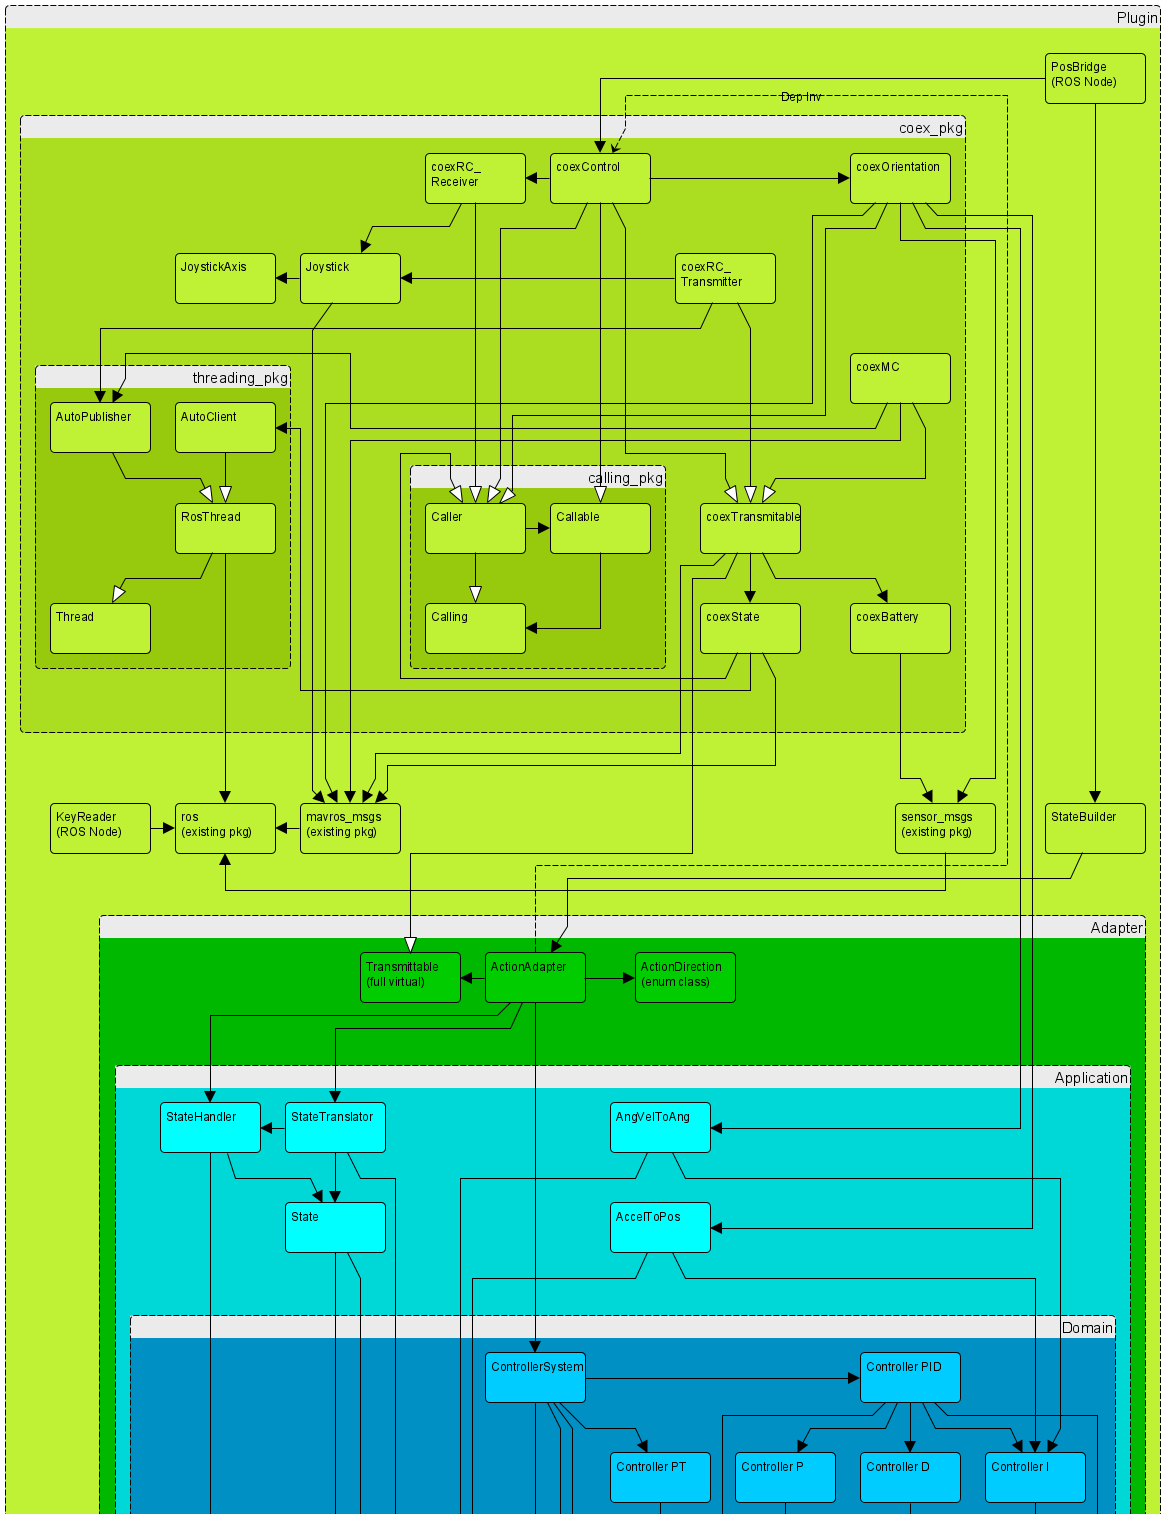
\includegraphics[width=15cm]{Pictures/Clean Architecture coex.png}}
\caption{Klassendiagramm des \textit{coex} \Pack[s]}
\label{fig:PackCoex}
\end{center}

\vspace{0.25cm}
Zur Veranschaulichung der Abhängigkeiten dieses Pakets soll \refImgShort{fig:PackCoex} dienen.
\end{figure}


\newSec{coexBattery}{4}
Wie der Klassenname vermuten lässt überwacht diese Klasse die Batteriestand des \Quad[s].
\\Diese Klasse entspricht der \CodeClass{parrotBattery} der \Ar.


\newSec{coexControl}{4}
Die \CodeClass{coexControl} ist als Fassade eingesetzt und bietet Anwendenden zugriff auf diverse Funktionen der gekapselten Klassen.
\\Diese Klasse entspricht der \CodeClass{parrotControl} der \Ar.


\newSec{coexMC}{4}
Die Abkürzung \textit{MC} im Klassennamen steht für \textit{Manual Control} und deutet hiermit sowohl das genutzte \Topic\ als auch den zugrundeliegenden Nachrichtentyp an. Laut Entwickler-Literatur (siehe \refCap{CoexLiteratur}) werden Steuerungsdaten der vier Freiheitsgrade an den \Quad\ gesendet. 

Diese Klasse erbt von der \CodeClass{coexTransmitable}
\\Diese Klasse entspricht der \CodeClass{parrotTransmitter} der \Ar.


\newSec{coexOrientation}{4}
Es war geplant, die Pose des \Quad[s] in dieser Klasse berechnen zu lassen. Im weiteren Projektverlauf hat sich ergeben, hierfür eine separate Klasse zu erstellen.
\\Diese Klasse entspricht der \CodeClass{parrotIMU} der \Ar.


\newSec{coexRC}{4}
Die \CodeClass{coexRC} ist als Fassade für die beiden nachfolgenden implementiert.


\newSec[coexRCR]{coexRC\_Receiver}{4}
Die \CodeClass{coexRC\_Receiver} liest vom \rTopic{/mavros/rc/in} und somit die Eingaben der Funkfernsteuerung. Eine nähere Erläuterung, welche Daten übermittelt werden, findet sich als Kommentar im Code.


\newSec[coexRCT]{coexRC\_Transmitter}{4}
Als \textit{RC-Transmitter} wird die Klasse bezeichnet, welche Nachrichten an das \rTopic{/mavros/rc/override} veröffentlicht (vgl. \refCap{COEXPkgTopic}).

Diese Klasse erbt von der \CodeClass{coexTransmitable}


\newSec{coexState}{4}
Die \CodeClass{coexState} übernimmt die Interaktion mit dem Zustandsautomaten, welcher im \textit{Flight Controller} des \Quad[s] realisiert ist.
Anfragen zur Änderung eies Zustand beziehen sich maßgeblich auf den Start und die Landung eines Flugs.
\\Diese Klasse entspricht der \CodeClass{parrotStatus} der \Ar.


\newSec{coexTransmitable}{4}
Diese Klasse erbt von der \CodeClass{Transmitable}. Hierin wird die Steuerung innerhalb dieses \Pack[s] als eine normierte \textit{Manual Control}-Nachricht mit dem Wertebereich [-1, 1] definiert.


\newSec{Joystick}{4}
Hier wird ein Hilfskonstrukt für die Transformation von Daten der Funkfernsteuerung eingeführt. Die Klasse implementiert vier Instanzen der \CodeClass{JoystickAxis}.


\newSec{JoystickAxis}{4}
Hier werden die Rohdaten der Kanäle der Funkfernsteuerung in normierte Daten zu überführt. Zudem können normierte Werte in den Wertebereich der Funkfernsteuerung transformiert werden.

